\section{Comparing Exclusion Limits between ML Models and Previous Analysis}
In the previous section I compared the achieved significance between 
the three optimal models for the full statistics signal set. In this section 
I will do the same, but with the introduction of a flat uncertainty in the background.
Additionally, I will compare the achieved exclusion limits (the mass combinations with an achieved 
significance of over 1.64) by the models created in this thesis, with the limit set in the paper by ATLAS 
in 2021 \cite{atlas_search_2021}.
\\
In the analysis by ATLAS, they have not assumed a flat uncertainty. Instead, an analysis has been made on the simulated data 
over individual regions and collision processes. Due to time constraints, a flat uncertainty has been made for comparison 
reasons. Aligning with what I have found when reading similar analysis (as well as based on recommendation from my supervisors), 
the uncertainty will be in the region of $20\%$ of the \ac{SM} background.\\
\begin{figure}
    \makebox[\linewidth][c]{%
    \centering
    \begin{subfigure}{.75\textwidth}
        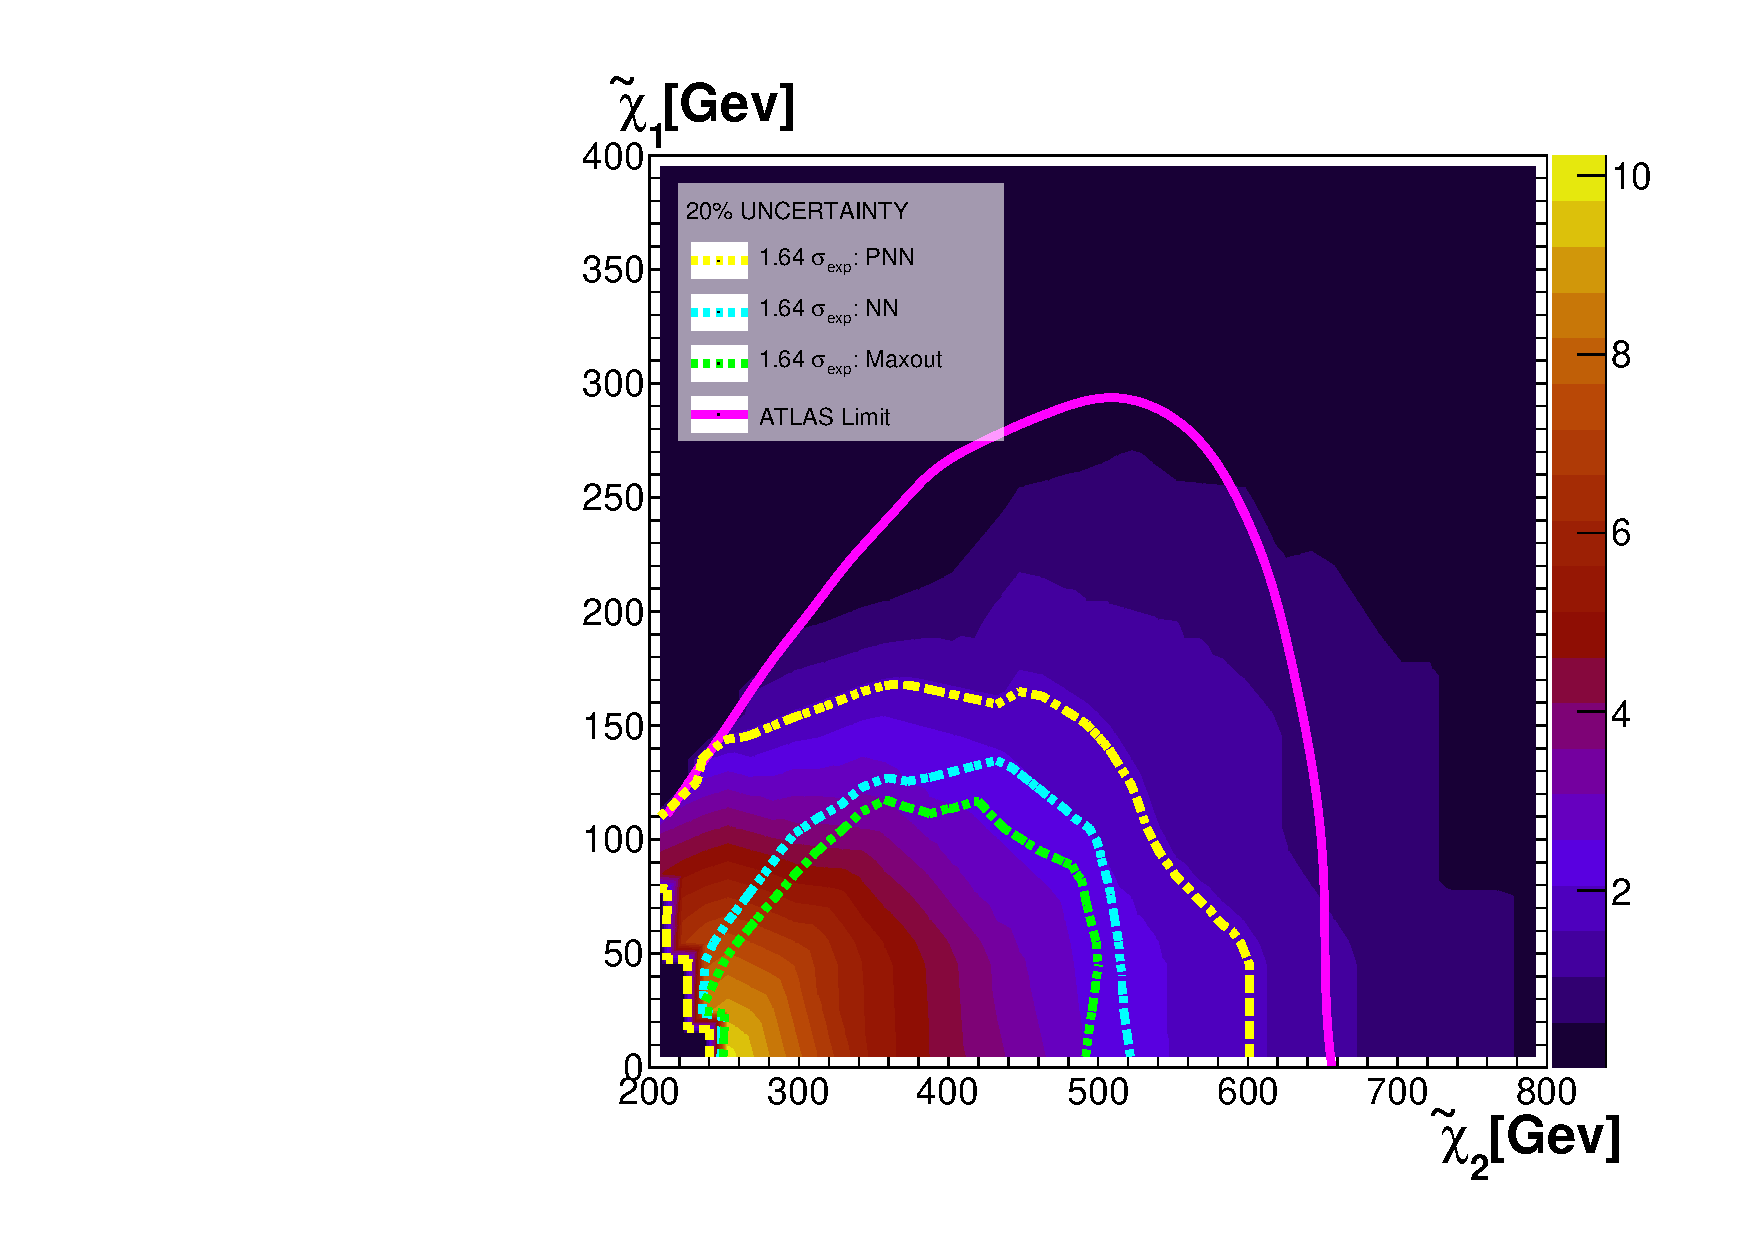
\includegraphics[width=\textwidth]{Figures/MLResults/NN/SUSY/Comparison/Limits/compLimit20.pdf}
    \end{subfigure}
    }
    \caption{A surface plot of the significance achieved by the \ac{PNN} on the full statistics signal set. Contours are 
    drawn around the band equal to a significance of 1.64 for the \ac{PNN} (yellow), dense \ac{NN} (cyan), maxout model (green)
    and the ATLAS analysis (pink). The significance achieved by the \ac{ML} models were calculated with a flat uncertainty equal 
    to $20\%$ of the background.}
    \label{fig:compLimit20}
\end{figure}
In figure \ref{fig:compLimit20}, I have drawn the contours of the significance achieved using the \ac{PNN},
while outlining all points corresponding to a significance of 1.64. The same outline has been made on top of the 
contours of the \ac{PNN} for the dense \ac{NN}, maxout model and the statistical analysis made by ATLAS. The calculations
of the significance for the output of the \ac{ML} models were made with a flat uncertainty equal to $20\%$ of the background.
The figure shows that none of the models are able to extend the sensitivity achieved by ATLAS, although the \ac{PNN} was able to equal
the ATLAS analysis for smaller masses. Furthermore, it is evident from the figure that the \ac{NN} and maxout model, were not able to 
extend the limit as far as the \ac{PNN}. In section \ref{sec:FS} I presented the achieved significance, calculated without uncertainty. In these
calculations the dense \ac{NN} and maxout model were able to extend the limit past that achieved by the \ac{PNN} (in certain areas). 
This contradiction can be explained by the fact that \ac{PNN} achieved a much higher sensitivity for smaller masses, in some cases even 
doubling the sensitivity to that of the dense \ac{NN} and maxout model. When introducing uncertainty, the \ac{NN} and maxout model are 
penalized for attempting to tune according to all signals, thereby not attaining enough sensitivity on the signals easiest to separate.
In contrast, the \ac{PNN}, although attempting to tune for all masses, includes the bias towards large statistics signals, which explains why there 
is less of a difference when comparing the limit with and without uncertainty.\\
\begin{figure}
    \makebox[1\linewidth][c]{%
    \centering
    \begin{subfigure}{.6\textwidth}
        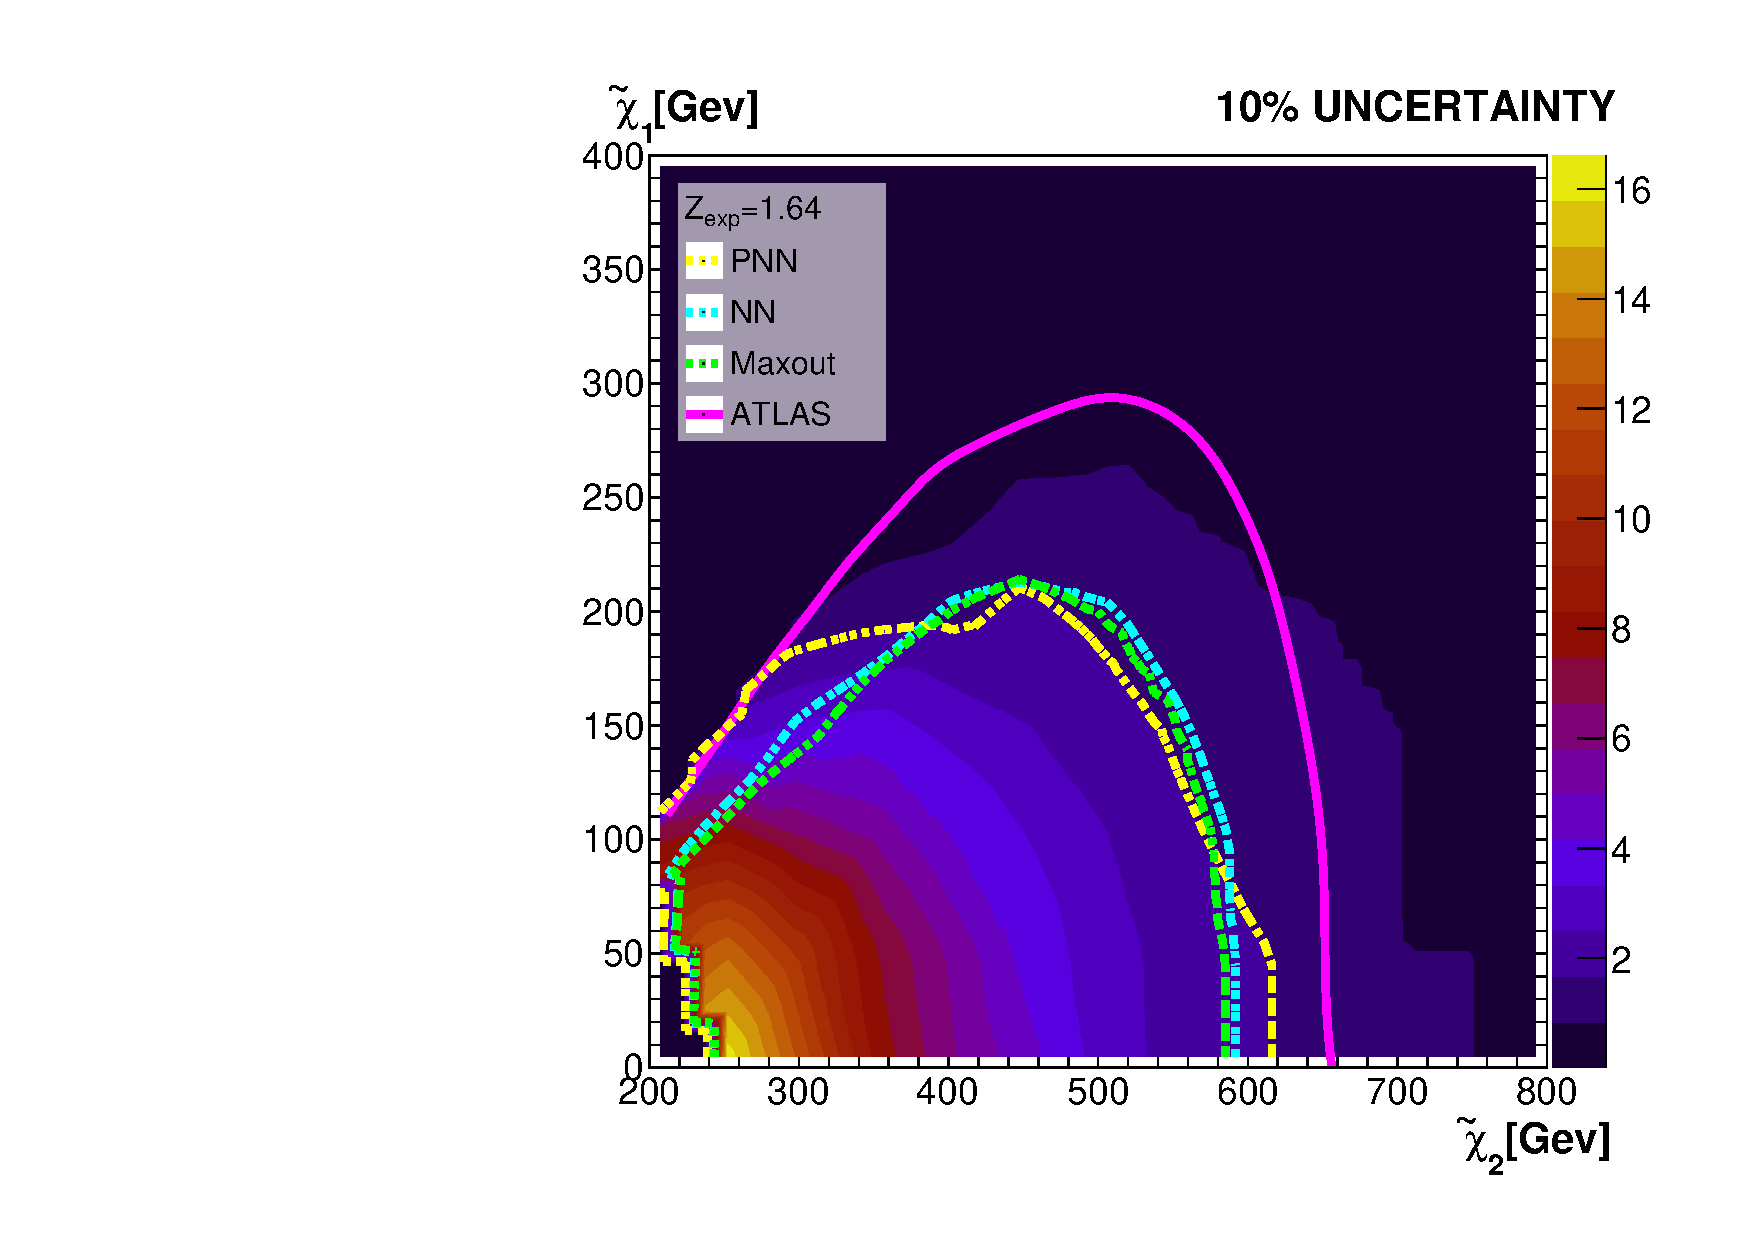
\includegraphics[width=\textwidth]{Figures/MLResults/NN/SUSY/Comparison/Limits/compLimit10.pdf}
        \vspace{-1.cm}
        \caption{}
        \label{fig:compLimit10}
    \end{subfigure}
    \begin{subfigure}{.6\textwidth}
        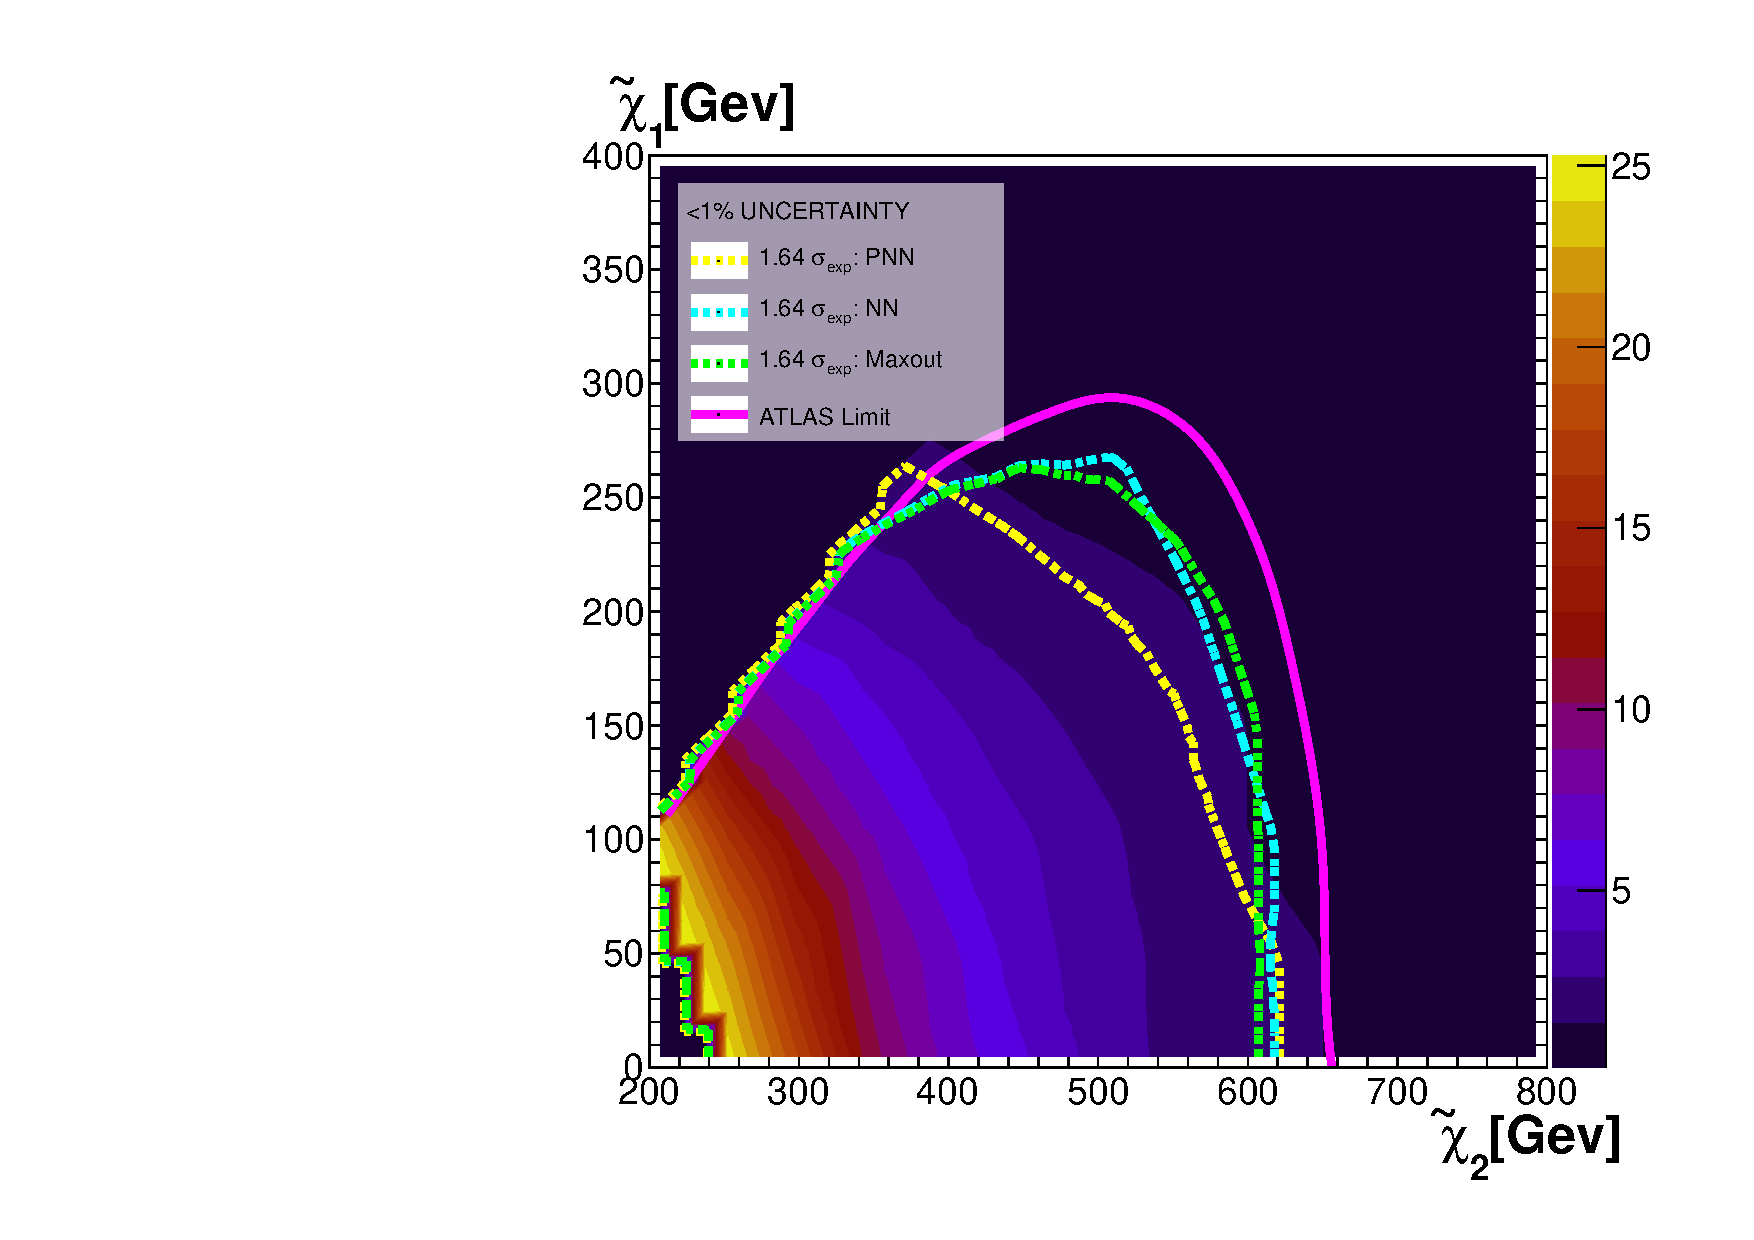
\includegraphics[width=\textwidth]{Figures/MLResults/NN/SUSY/Comparison/Limits/compLimit1.pdf}
        \vspace{-1.cm}
        \caption{}
        \label{fig:compLimit1}
    \end{subfigure}
    }
    \caption{Two surface plots of the significance achieved by the \ac{PNN} on the full statistics signal set. Contours are 
    drawn around the band equal to a significance of 1.64 for the \ac{PNN} (yellow), dense \ac{NN} (cyan), maxout model (green)
    and the ATLAS analysis (pink). The significance achieved by the \ac{ML} models were calculated with a flat uncertainty equal 
    to $10\%$ of the background in the left figure \ref{fig:compLimit10} and less than $1\%$ in the right \ref{fig:compLimit1}.}
\end{figure}
To further study the sensitivity of the models, I produced two additional figures similar to the one above. In these figure I applied an uncertainty of 
$10\%$ (\ref{fig:compLimit10}) and less than $1\%$ (\ref{fig:compLimit1}) of the background. As expected, the limits converge close towards the limits 
observed in section \ref{sec:FS} for smaller uncertainties. In figure \ref{fig:compLimit10}, we even discern that the limits set by the dense \ac{NN}
and maxout model even extend past the \ac{PNN}, for high masses of both $\tilde{\chi}_1$ and $\tilde{\chi}_2$, although it is beaten for most other combinations.
In figure \ref{fig:compLimit1}, I chose a sensitivity close to 0. In this figure, we observe that the dense \ac{NN} and maxout model 
very closely resemble the limits from ATLAS, only being beaten by $50GeV$ for high masses $\tilde{\chi}_2$. In the mass region of
$\tilde{\chi}_1\approx250GeV$ and $\tilde{\chi}_2\approx400GeV$, the \ac{PNN} seems to ever so slightly extend the limit surpassed that produced of ATLAS.
Although this is promising for the method, it is worth mentioning that the uncertainty is far from realistic. Finally, the size by which the limit are extended
are so small that it could be explained by the method of interpolation between the grid of mass combinations.
\subsection*{Final Remarks and Possible Improvements}
To summarize the discoveries in the figures above, none of the methods were able to extend the limit passed that produced by ATLAS, at least not to a satisfactory degree.
This is by no means to say that the methods discussed and presented in this thesis are not of interest. For starters, the matter of trying to extend the limit of sensitivity 
passed that produced by ATLAS, was given little attention and consideration during the timespan of this thesis. Most of the time, was instead spent comparing and exploring the 
different models. In contrast, limit set by ATLAS is the result of a large team of focused scientist all attempting to push the limit as far as they can. This considered, I believe 
the models to show great promise. If I were to prioritize expansion of exclusion limits, there are several aspects of the analysis in this thesis I would improve.
\begin{itemize}
    \item \emph{A more advanced analysis of the signal region}: In my analysis, I chose to define the signal regions from each model's output using a brute force approach. 
          A more advanced approach, applying optimization technics to find the maximum possible significance from each output, would most likely produce a higher sensitivity.
    \item \emph{Devote additional time to studying the relationship between overfitting and significance}: The early stoppage criteria of 10 epochs applied in this analysis, was chosen 
          for convenience and was based on general practice. This rigid criteria, could be destructive for optimal performance, and by devoting additional time to studying
          the relationship between the threshold for the criteria and optimal performance could lead to better performing models.
    \item \emph{Perform a thorough hyperparameter search}: For comparison reasons, I decided not to apply a hyperparameter search for the architecture of the networks. By attempting 
           a grid search for the different hyperparameter, it would be interesting to see if a better performance could be achieved. Additionally, attempting to combine the methods presented 
           in this thesis, for example a \ac{PNN} with maxout layers. 
    \item \emph{Create region specific models}: In the final analysis, I applied one model (per method) to study the full signal set. It would be interesting to explore the possibility of creating
          different models for different regions in the feature space. In the analysis we have seen how models can both improve and worsen in performance with regard to specific masses by increasing
          the number of mass combinations in the training set. With individual models covering specific, possibly physics motivated regions, I believe some methods would benefit.
    \item \emph{Focus on relevant regions}: In this analysis I have treated the performance of a model on all mass combinations equally. This was a choice I made to easier compare methods, but 
          given the goal of extending the limits, it would most likely be beneficial to prioritize the regions closest to the existing limits, in hopes of achieving a higher sensitivity in these 
          regions\footnote{See the final paragraph in section \ref{sec:PCA}}.  
\end{itemize}

